\documentclass[12pt,a4paper]{article} 

\usepackage[utf8]{inputenc}
\usepackage[margin=1.3cm]{geometry}
\usepackage[francais]{babel} 
\usepackage{amsfonts} 
\usepackage{graphicx} 
\usepackage{amsmath} 
\setlength{\unitlength}{1mm}
\usepackage{enumitem}
\usepackage{cancel}
\usepackage{fancyhdr}
\usepackage{fancybox}
\usepackage{hyperref}
\usepackage{array}
\usepackage{titling}
\usepackage{stmaryrd}
\usepackage{graphicx}
\usepackage{wrapfig}
\usepackage{algorithm}
\usepackage{algpseudocode}
\graphicspath{ {./images/} }

\makeatletter
\renewcommand{\ALG@name}{Algorithme}

\algblock{Input}{EndInput}
\algnotext{EndInput}


\lhead{Antoine Groudiev}
\chead{}
\rhead{MP*, Charlemange}

\lfoot{\jobname.tex}
\cfoot{Calcul de distance}
\rfoot{\thepage}
\renewcommand{\headrulewidth}{0.4pt}
\renewcommand{\footrulewidth}{0.4pt}

\author{Antoine Groudiev - n°15039}
\title{Vision par ordinateur appliquée à la détection de panneaux}

\begin{document}
\maketitle

\section*{Introduction}
La détection d'objets est la branche de la vision par ordinateur visant à classifier des images selon la présence ou l'absence d'un objet spécifique dans l'image. Je me suis intéressé à la détection de panneaux routiers dans un flux vidéo, et plus spécifiquement à un algorithme de \textit{boosting}. Le terme \textit{boosting} désigne une famille d'algorithmes d'apprentissage qui pondère un ensemble de classificateurs faibles, qui classent chacun légèrement mieux que le hasard, pour former un classificateur fort de bonne exactitude.

\section{Algorithme de Viola et Jones}
\textit{AdaBoost} est un des algorithmes de \textit{boosting} les plus populaires, notamment grâce à son utilisation par la méthode de Viola et Jones, un algorithme de reconnaissance de visages, présenté en 2001 \cite{viola-jones}.

Le détecteur doit pouvoir prendre en entrée des images de tailles quelconques, et retourner la liste des emplacements dans l'image de l'objet à détecter. La première phase de la création du détecteur se restreint cependant à la détection d'objets dans une image carrée de petite taille : j'ai fait le choix de \texttt{19px} de côté. La dernière partie de l'algorithme, détaillée en \ref{sec:taille_standard}, appliquera ce détecteur à une image detaille standard, i.e. de plusieurs centaines de pixels de côté.

\subsection{Classificateurs faibles}
La méthode de \textit{boosting} fonctionne par la sélection de classificateurs faibles. Dans le contexte de la méthode de Viola et Jones, un classificateur faible est constitué de trois éléments.

\subsubsection{Les \textit{features}}
Une \textit{feature} est consitutée de $2$ à $4$ régions rectangulaires adjacentes, comptées positivement ou négativement. Leur forme est imposée comme dans la figure ... . 

\begin{figure}[t]
    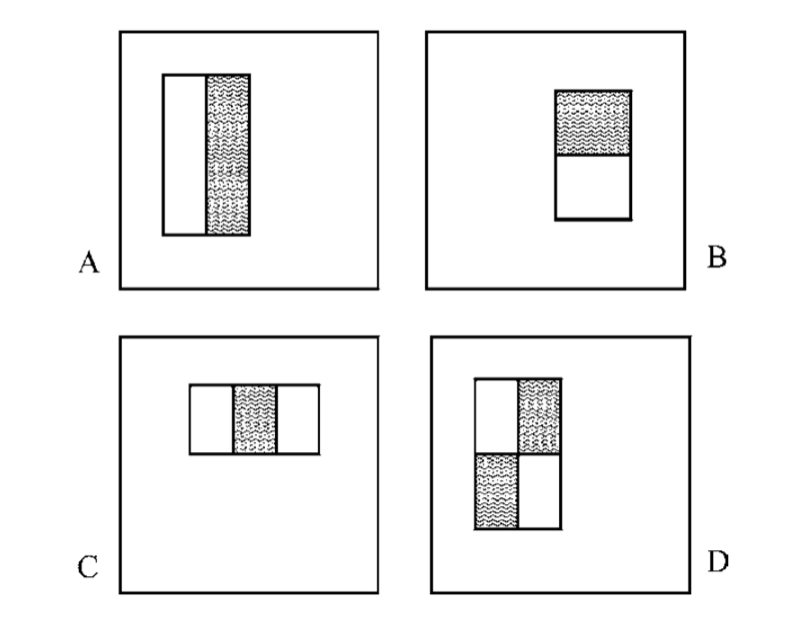
\includegraphics[scale = 0.4]{forme_features}
    \centering
    \caption{Forme des \textit{features}}
\end{figure}

Chaque \textit{feature} va cibler une zone spécifique de l'objet à détecter. Dans le cas d'un visage par exemple, le détecteur peut apprendre que la zone du creux de l'oeil est généralement plus sombre que la zone entre les deux yeux. Ainsi, une image comportant cette différence de luminosité caractéristique sera probablement un visage.


Chaque \textit{feature} peut être évaluée sur l'image à l'aide de la formule suivante (le score le plus faible étant le meilleur) :
$$formule$$
Ainsi, le score d'une \textit{feature} est d'autant plus faible que les zones positives compensent les zones négatives. 


Le nombre de \textit{features} possibles croît exponentiellement avec le côté de l'image, d'où la nécessité d'entraîner dans un premier temps un détecteur de côté faible.

%\begin{wrapfigure}{r}{0.5\textwidth}
\begin{figure}[t]
    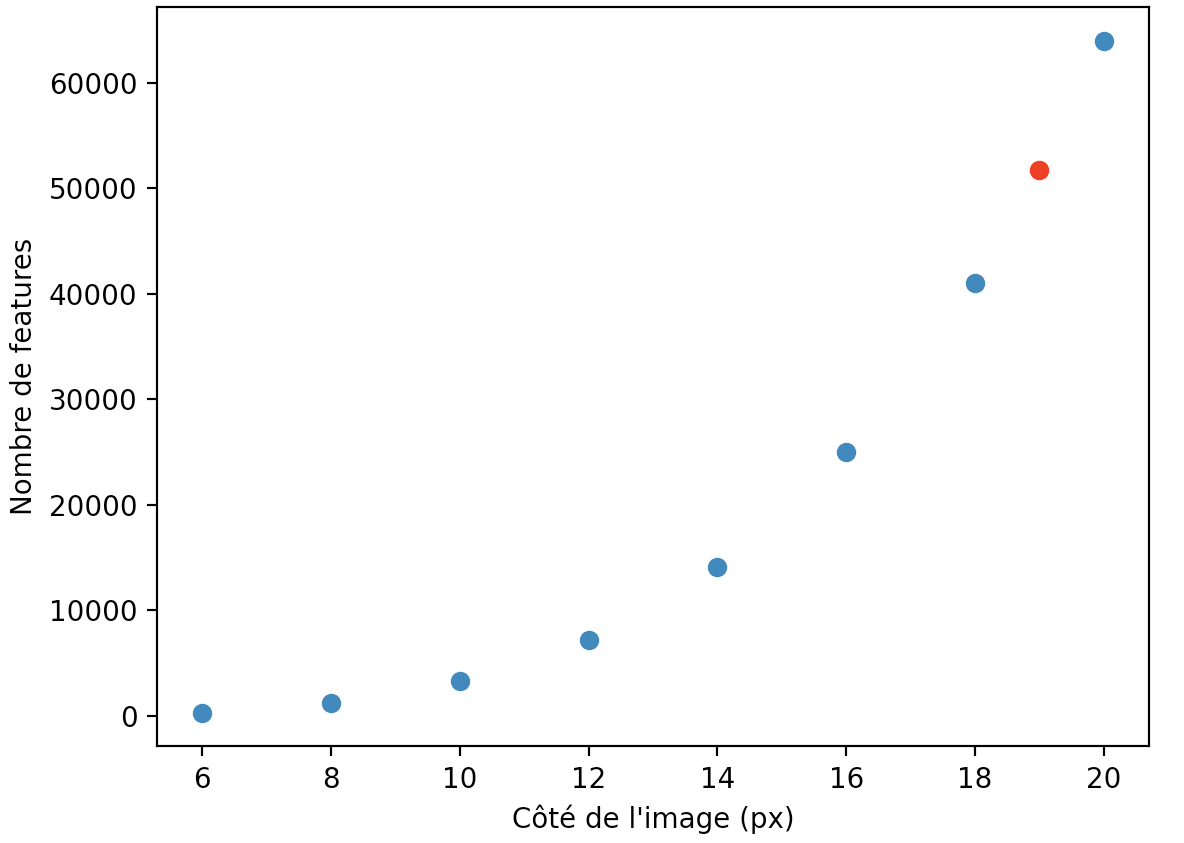
\includegraphics[scale = 0.4]{nombre_features_cut}
    \centering
    \caption{Nombre de \textit{features} en fonction de la taille de l'image}
\end{figure}
%\end{wrapfigure}

\subsubsection{Évaluation par un classificateur faible}
À chaque \textit{feature} notée $f$ est associée un \textit{threshold} (ou seuil) $\theta > 0$, et une polarité $p \in \{-1 ; 1\}$. Soit $x$ une image de \texttt{19px} de côté. Le classificateur faible $C_{(f, \: \theta, \: p)}^{faible}$ convertit le score de la \textit{feature} sur $x$ en un booléen selon la loi suivante :
$$C_{(f, \: \theta, \: p)}^{faible}(x) = 
\begin{cases}
1 \:\: si \:\: pf(x) < p\theta \\
0 \:\: sinon
\end{cases}$$
Si le score de la \textit{feature} sur $x$ est, à la polarité près, sous le seuil, alors le classificateur faible juge que la zone de l'image correspond à l'objet à détecter.

\subsection{Image intégrale}
La complexité du calcul du score d'un classificateur faible est déterminée par la complexité du calcul de la somme des valeurs des pixels dans un sous-rectangle de l'image.

Une approche naïve consisterait à recalculer, à chaque évaluation du score d'un classificateur, la somme des valeurs des pixels de l'image dans certaines de ses régions rectangulaires. Un tel calcul pour une région de taille $L_r$ sur $l_r$ a une complexité en $O(L_r \times l_r)$. Si l'on considère une image de dimensions $n \times n$ et que l'on veut calculer la somme dans $p$ régions de dimensions proches de $n \times n$, la complexité totale est en $O(p \times n^2)$.

Pour réduire cette complexité, la méthode de Viola et Jones introduit \textbf{l'image intégrale}. Si l'image considérée est $(i(x, y))$, alors l'image intégrale, notée $(ii(x, y))$ vérifie :
$$\forall x, y, ii(x, y) = \sum_{x' \leq x, y' \leq y} i(x', y')$$
Ainsi, chaque coefficient de l'image intégrale contient la somme des coefficients en haut à gauche du pixel considéré. Ceci permet alors d'accéder en temps constant à la somme des pixels dans un sous-rectangle de l'image $(i(x, y))_{x, y}$, en réalisant simplement la somme de quatre termes.

\begin{figure}[t]
    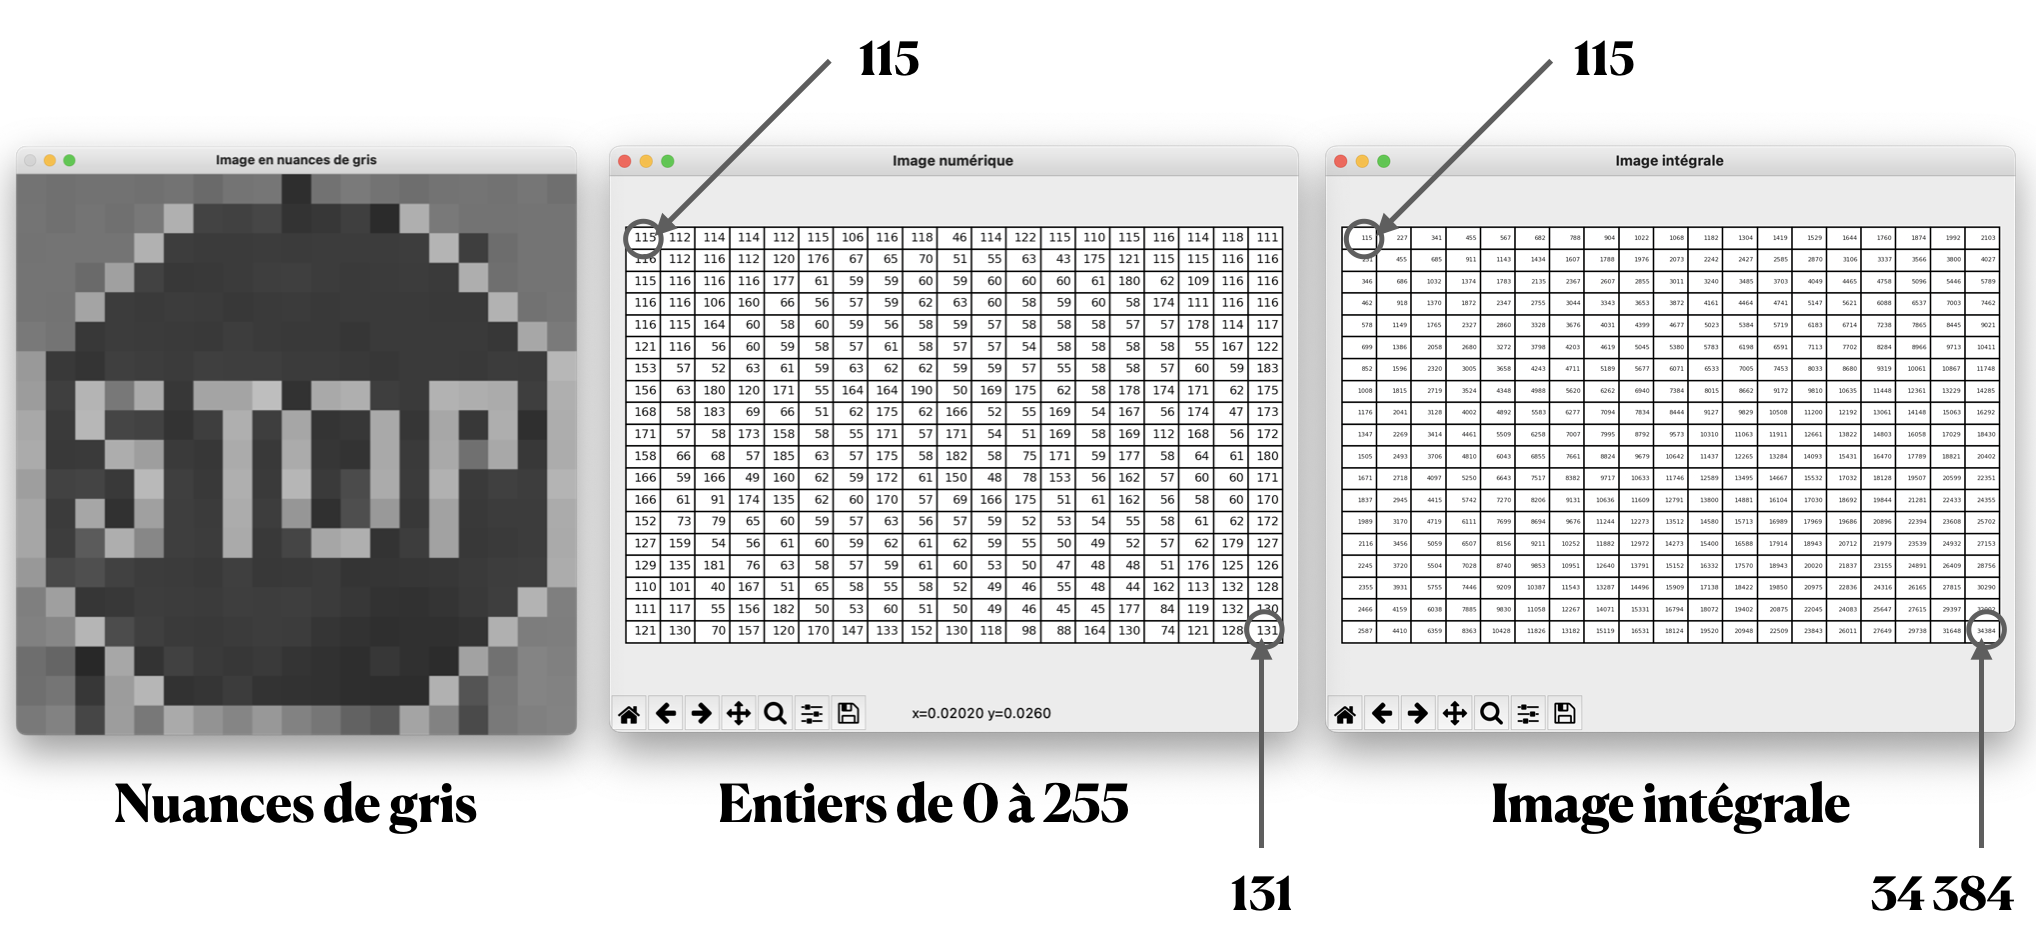
\includegraphics[scale = 0.35]{image_integrale}
    \centering
    \caption{Une image, sa représentation en mémoire, et son image intégrale}
\end{figure}


\subsection{Sélection des caractéristiques par \textit{AdaBoost}}
La phase de \textit{boosting} à proprement parler vise à sélectionner un nombre $T \in \mathbb{N}^*$ de classificateurs faibles qui représentent le mieux l'objet à détecter. L'algorithme utilise pour cela en entrée un jeu d'entraînement, c'est-à-dire une liste de tuples $(x, y) \in \mathcal{M}_{19, 19}(\llbracket 0, 255 \rrbracket) \times \{0 ; 1\}$. Chaque tuple est constitué d'une image contenant ou ne contenant pas l'objet à détecter, centré et cadré le cas échéant, et d'un label booléen, valant $1$ si l'objet à détecter est effectivement représenté sur l'image. La constitution d'un tel jeu sera détaillée en \ref{sec:pre-traitement}.

\begin{figure}[t]
    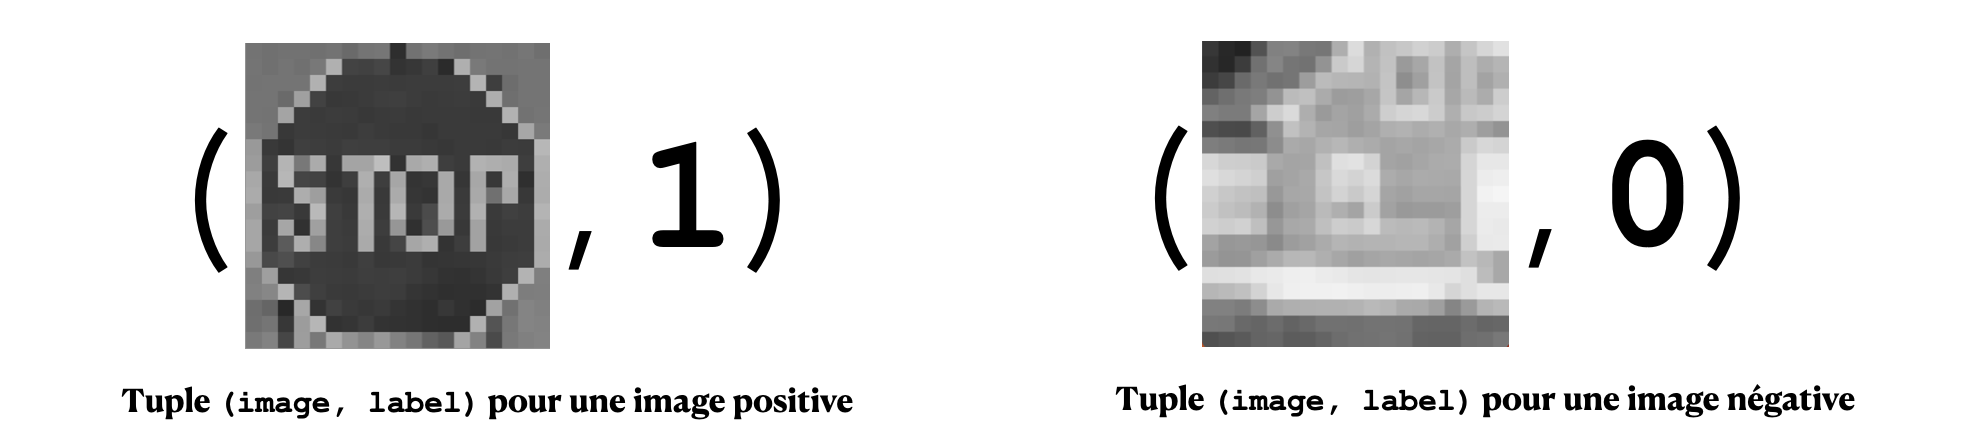
\includegraphics[scale = 0.5]{exemples_jeu}
    \centering
    \caption{Exemple de deux tuples du jeu d'entraînement}
\end{figure}

L'algorithme \textit{AdaBoost} est un algorithme glouton qui sélectionne un à un les $T$ meilleurs classificateurs parmi les $50\,000$ présents dans l'image de \texttt{19px} de côté. 

En toute généralité, la complexité de \textit{AdaBoost} est en $O(n \cdot F \cdot \tau + T \cdot n)$ où $n$ désigne le nombre d'images d'entraînement, $F$ le nombre total de classificateurs faibles, et $\tau$ le temps moyen de classification d'un classificateur faible sur un $x_i$. On a $T = O(F)$ et dans le cas de Viola-Jones, l'image intégrale garantit $\tau = O(1)$, ce qui donne une complexité en $O(n \cdot F)$.

Après sélection des $T$ classificateurs faibles, l'algorithme les combine en un unique classificateur fort $C^{fort}$, défini par :

$$C_T^{fort}(x) = 
\begin{cases}
1 \:\: si \:\: \sum_{i=1}^T \alpha_i C_i^{faible}(x) \leq \frac{1}{2} \sum_{i=1}^T \alpha_i \\
0 \:\: sinon
\end{cases}$$

où les $\alpha_i = \log(\frac{1 - \varepsilon_i}{\varepsilon_i})$ pondèrent les classificateurs selon leur erreur. Ainsi, aux pondérations près, si au moins la moitié des classificateurs faibles valent $1$, le classificateur fort vaut $1$.

%\begin{wrapfigure}{L}{0.6\textwidth}
%\begin{minipage}{0.6\textwidth}
\begin{algorithm}[H]
    \caption{Entraînement par AdaBoost}
    \begin{algorithmic}
        \Input

        $(x_1, y_2), ..., (x_n, y_n)$
        \Comment{Jeu d'entraînement}
        \EndInput
        \State $m \gets$ nombre d'images négatives
        \State $l \gets$ nombre d'images positives
        \For{$i \in \llbracket 1, n \rrbracket$} \Comment{Initialisation des poids}

            \State $w_{1, i} \gets \begin{cases}
                \frac{1}{m} \:\: si \:\: y_i = 0 \\
                \frac{1}{l} \:\: sinon
                \end{cases}$
        \EndFor
        \For{$t \in \llbracket 1, T \rrbracket$}

            \State Normaliser les poids : $w_{t, i} \gets \frac{w_{t, i}}{\sum_{j=1}^n w_{t, j}}$

            \For{$i \in \llbracket 1,$ nombre de classificateurs $\rrbracket$}

                \State $\varepsilon_i = \sum_i w_{t,i} \times \delta(C_i^{faible}(x_i), \overline{y_i})$ \Comment{Calcul de l'erreur de chaque classificateur}
            \EndFor

            \State $C_t^{faible} \gets \arg \min_i \varepsilon_i$
            \For{$i \in \llbracket 1, n \rrbracket$} \Comment{Mise à jour des poids}

            \If{image $x_i$ bien classée par $C_t^{faible}$}
                \State $w_{t+1, i} \gets w_{t, i} \times \frac{\varepsilon_t}{1- \varepsilon_t}$ \Comment{le poids baisse à $t+1$}

            \Else
                \State $w_{t+1, i} \gets w_{t, i}$ \Comment{le poids augmente à $t+1$}
            \EndIf
        \EndFor
        \EndFor
    \end{algorithmic}
\end{algorithm}
%\end{minipage}
%\end{wrapfigure}

\subsection{Mise en cascade}
Selon sa valeur de $T$, un classificateur fort est soit très efficace (pour $T$ faible), soit très exact (pour $T$ élevé). L'introduction du concept de cascade permet d'allier exactitude et efficacité. 

\begin{figure}[t]
    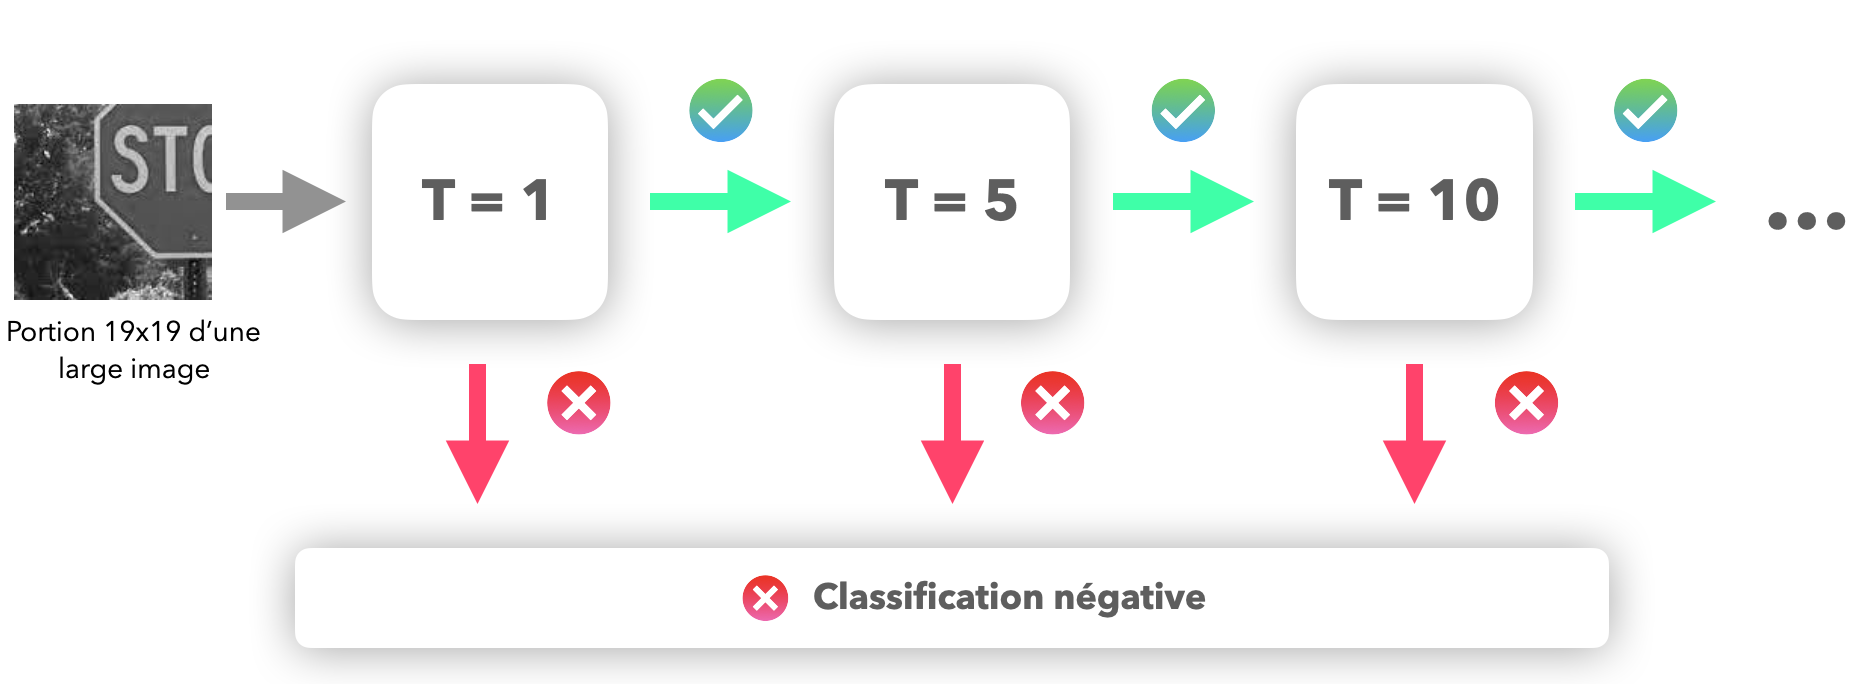
\includegraphics[scale = 0.5]{cascade}
    \centering
    \caption{Schéma d'une cascade}
\end{figure}

Une image analysée par la cascade va être classée successivement par une suite $(C_T^{fort})_T$ pour des valeurs de $T$ croissantes. Une image est alors rejetée par la cascade dès qu'elle est classée négativement par un des classificateurs forts, permettant une grande efficacité. Au contraire, une image finalement classée positivement par la cascade sera passée à travers des classificateurs forts avec $T$ très grands, garantissant un faible nombre de faux positifs.

\subsection{Application à des images de taille standard}
\label{sec:taille_standard}



\section{Pré-traitement des images d'entaînement et de test}
\label{sec:pre-traitement}

\section{Mesure de l'exactitude et de l'efficacité de l'implémentation}
Le langage courant confond l'exactitude, c'est à dire la proximité du résultat expérimental à la valeur théorique, et la précision, qui quantifie la dispersion des résultats. L'objectif de cette dernière partie vise à déterminer précisément l'exactitude du détecteur précédement implémenté.

\subsection{Quantification de l'exactitude}
Posons :
\begin{enumerate}
    \item $V_p$, le nombre de vrais positifs (i.e. images positives classées positivement)
    \item $V_n$, le nombre de vrais négatifs (i.e. images négatives classées négativement)
    \item $F_p$, le nombre de faux positifs (i.e. images négatives classées positivement)
    \item $F_n$, le nombre de faux négatifs (i.e. images positives classées négativement)
\end{enumerate}

\subsubsection{Approche standard}
Il semble intuitif de poser l'exactitude comme étant :
$$ A = \frac{bons\ classements}{total} $$
Ou encore avec les notations introduites précédement :
$$\boxed{A = \frac{V_p + V_n}{V_P + V_n + F_p + F_n}}$$

Cependant, cette méthode de calcul introduit des biais en cas de déséquilibre important entre le nombre d'images positives et le nombre d'images négatives. Nos échantillons de tests étant fortement déséqulibrés, il faut introduire une nouvelle méthode de calcul de l'exactitude.

\subsubsection{F-Score}
On utilise alors le F-Score ou $F_1$-Score, défini comme la moyenne harmonique de la précision et du rappel.

La précision est définie comme :
$$ P = \frac{bons\ classements}{classements\ positifs} = \boxed{\frac{V_p}{V_P + F_p}} $$

Le rappel est défini comme :
$$ R = \frac{bons\ classements}{images\ positives} = \boxed{\frac{V_p}{V_P + F_n}} $$

Finalement, l'exactitude est calculée comme la moyenne harmonique des deux :
$$\boxed{A = \frac{2}{\frac{1}{P} + \frac{1}{R}} = \frac{2 P R}{P+R}}$$


\subsection{Résultats du détecteur de \texttt{19px}}
\subsection{Résultats du détecteur de taille standard}

\section{Annexes}
\subsection{Complexité de l'image intégrale}
On introduit les deux suites suivantes, calculées par récurrence :
$$s(x, y) = s(x, y-1) + i(x, y)$$
$$ii(x, y) = ii(x-1, y) + s(x, y)$$

initialisées par $s(x, -1) = 0$, $ii(-1, y) = 0$. Ceci permet de calculer $(ii)$ avec une complexité linéaire en le nombre de pixels de l'image, soit la même complexité que pour le seul calcul de la somme de tous les pixels dans l'image, correspondant au sous-rectangle maximal.

\begin{thebibliography}{5}
    
    \bibitem{szeliski}Richard Szeliski, \textit{Computer Vision: Algorithms and Applications, 2nd ed. (2022)}, \url{https://szeliski.org/Book/}
    \bibitem{viola-jones}Paul Viola, Michael Jones, \textit{Rapid Object Detection using a Boosted Cascade of Simple Features}, Conference on Computer Vision and Pattern Recognition, \url{https://www.cs.cmu.edu/~efros/courses/LBMV07/Papers/viola-cvpr-01.pdf}
    \bibitem{computerphile}Michael Pound, Sean Riley, Computerphile, \textit{Detecting Faces (Viola Jones Algorithm)}, \url{https://www.youtube.com/watch?v=uEJ71VlUmMQ&t=15s}
    \bibitem{wang}Yi-Qing Wang, \textit{An Analysis of the Viola-Jones Face Detection Algorithm}, IPOL, \url{https://www.ipol.im/pub/art/2014/104/?utm_source=doi}
    %\bibitem{parande}Anmol Parande, \textit{Understanding and Implementing the Viola-Jones Image Classification Algorithm}, Medium, DataDrivenInvestors, \url{https://medium.datadriveninvestor.com/understanding-and-implementing-the-viola-jones-image-classification-algorithm-85621f7fe20b}
    \bibitem{powers}David M W Powers, \textit{Evaluation: From Precision, Recall and F-Measure to ROC, Informedness, Markedness \& Correlation}, Journal of Machine Learning Technologies,  \url{https://web.archive.org/web/20191114213255/https://www.flinders.edu.au/science_engineering/fms/School-CSEM/publications/tech_reps-research_artfcts/TRRA_2007.pdf}


\end{thebibliography}

\end{document}